Se implementó un modelo de autoencoder como parte de una estrategia de aprendizaje no supervisado para predecir y entender el comportamiento del usuario a partir de un conjunto de datos complejo.

\subsection{Preprocesamiento y Preparación de Datos}

Iniciamos con la carga del dataset desde un archivo CSV, seguido por una fase de limpieza de datos para garantizar la calidad del entrenamiento. Se realizaron las siguientes operaciones de preprocesamiento en los datos.

\subsection{Codificación One-Hot}

Se transformaron las variables categóricas 'método' y 'canal' en representaciones numéricas que son adecuadas para el procesamiento del modelo.

\begin{itemize}
    \item \textbf{Normalización de Fechas:} La columna 'fecha\_evento', que contenía información de fecha y hora, se dividió y estandarizó para asegurar un formato uniforme y utilizable.
    \item \textbf{Eliminación de columnas innecesarias:} Las columnas originales de 'método' y 'canal' se eliminaron después de la codificación, manteniendo el dataset conciso y enfocado en las características relevantes.
    \item \textbf{Transformación Temporal Adicional:} Se llevaron a cabo codificaciones one-hot para las columnas de 'fecha', 'hora' y 'día de la semana', ampliando la representatividad de los aspectos temporales de los datos.
\end{itemize}

\begin{figure}[H]
    \begin{minipage}[t]{0.9\textwidth}
        \caption{Preparación y codificación one-hot de los datos}
        \label{codificación_autoencoder}        
    \end{minipage}

    \vspace{10pt}

    \begin{minipage}[b]{0.9\textwidth}
        \centering
        \includegraphics[width=\textwidth]{img/codificación one-hhot.jpg}        
    \end{minipage}

    \begin{minipage}[t]{0.9\textwidth}
        Fuente: Elaboración propia.
    \end{minipage}
\end{figure}


\subsection{Construcción y Entrenamiento del Modelo}

El dataset fue dividido en conjuntos de entrenamiento y validación. Luego, se construyó la arquitectura del autoencoder con capas densas y normalización por lotes, utilizando una función de activación 'tanh' para las capas codificadoras y 'relu' para las decodificadoras. Se implementó un mecanismo de EarlyStopping para prevenir el sobreentrenamiento y mejorar la generalización del modelo.

\begin{figure}[H]
    \begin{minipage}[t]{0.9\textwidth}
        \caption{Arquitectura del modelo autoencoder}
        \label{arquitectura_autoencoder}        
    \end{minipage}

    \vspace{10pt}

    \begin{minipage}[b]{0.99\textwidth}
        \centering
        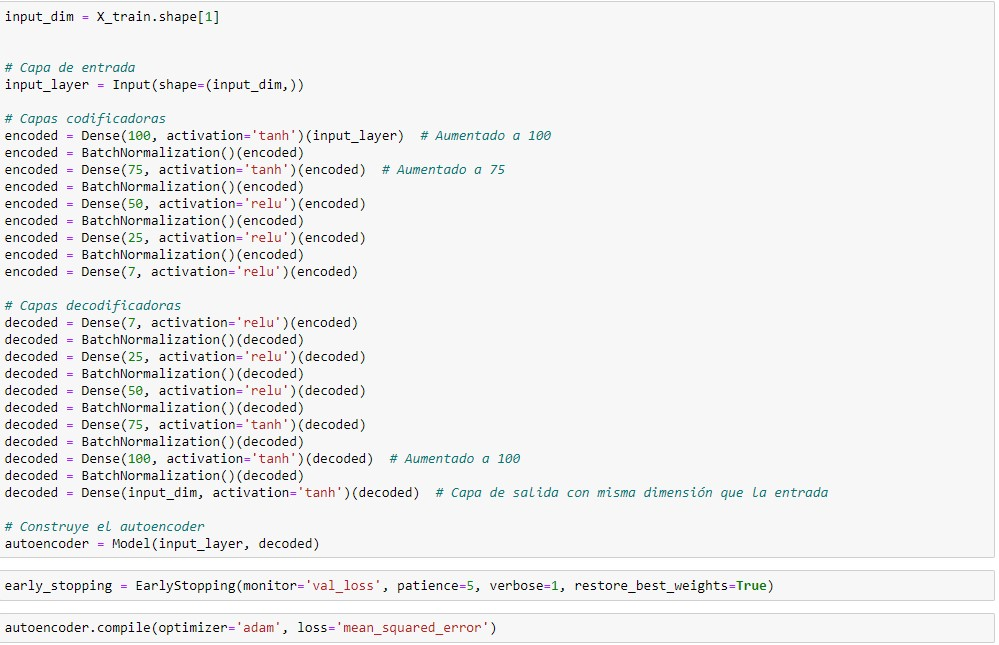
\includegraphics[width=\textwidth]{img/Arquitectura modelo autoencoder.jpg}        
    \end{minipage}

    \begin{minipage}[t]{0.9\textwidth}
        Fuente: Elaboración propia.
    \end{minipage}
\end{figure}

El entrenamiento se realizó con un enfoque iterativo, monitoreando la pérdida de validación para ajustes durante el proceso. Los resultados se visualizaron mediante gráficos de pérdida a lo largo de las épocas, lo que demostró una disminución constante de la pérdida y un modelo bien ajustado.

\begin{figure}[H]
    \begin{minipage}[t]{0.9\textwidth}
        \caption{Entrenamiento del modelo autoencoder}
        \label{entrenamiento_autoencoder}        
    \end{minipage}

    \vspace{10pt}

    \begin{minipage}[b]{0.99\textwidth}
        \centering
        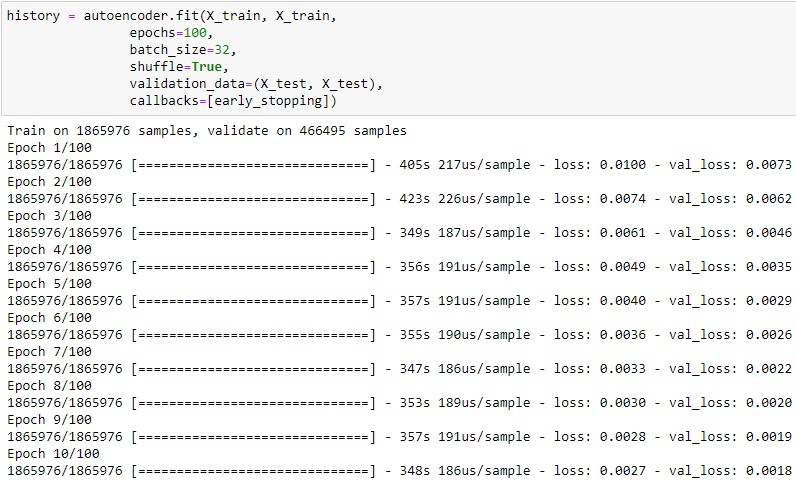
\includegraphics[width=\textwidth]{img/Entrenamiento autoencoder.jpg}        
    \end{minipage}

    \begin{minipage}[t]{0.9\textwidth}
        Fuente: Elaboración propia.
    \end{minipage}
\end{figure}

\subsection{Resultados y Evaluación}

El modelo final demostró una sólida capacidad de reconstrucción y no mostró signos de sobreajuste, como se evidencia en los gráficos de pérdida de entrenamiento. Este autoencoder está ahora listo para ser utilizado para transformar los datos en una representación de menor dimensión, lo cual facilitará la aplicación de técnicas de clustering para la segmentación de usuarios y la detección de patrones de comportamiento anómalos.

\begin{figure}[H]
    \begin{minipage}[t]{0.9\textwidth}
        \caption{Gráfico del entrenamiento del modelo autoencoder}
        \label{gráfico_autoencoder}        
    \end{minipage}

    \vspace{10pt}

    \begin{minipage}[b]{0.9\textwidth}
        \centering
        \includegraphics[width=\textwidth]{img/Gráfico entrenamiento autoencoder.png}        
    \end{minipage}

    \begin{minipage}[t]{0.9\textwidth}
        Fuente: Elaboración propia.
    \end{minipage}
\end{figure}

\subsection{Conclusión del Modelo de Autoencoder}

El autoencoder se diseñó para transformar datos de alta dimensión en una representación de menor dimensionalidad, lo cual es un paso fundamental en el pre-procesamiento para algoritmos de clustering.

Sin embargo, el propósito inicial del autoencoder no era predecir comportamientos futuros o tendencias, sino más bien identificar patrones intrínsecos y datos atípicos dentro del conjunto de datos existente. Dado que el objetivo central del proyecto es la predicción del comportamiento, se ha determinado que el autoencoder no cumple con los requisitos necesarios para avanzar hacia este nuevo objetivo.

Por tanto, hemos decidido no continuar con el desarrollo e implementación de este modelo en su forma actual. En cambio, nos enfocaremos en la búsqueda y aplicación de modelos predictivos más adecuados que estén alineados con las metas de pronosticar el comportamiento futuro y que puedan ofrecer insights más directos para la toma de decisiones y estrategias proactivas.

Este cambio de dirección subraya la importancia de una alineación clara entre las herramientas de modelado seleccionadas y los objetivos específicos del proyecto. Aunque el autoencoder es una herramienta poderosa para ciertas aplicaciones, en este caso, se ha reconocido que no es la solución óptima para las necesidades proyectadas.

Sin embargo, es importante destacar que el autoencoder es una herramienta extremadamente útil para identificar anomalías en patrones de comportamiento.
